\subsubsection{Diseño del contenedor}

Al final de trabajo terminal 1, se había propuesto utilizar un contenedor de acero laminado en frío, el cual cuenta con las características necesarias para el compostador, pues es resistente a las altas temperaturas, al óxido y menos propenso a ser dañado por alguna plaga. 
Y a diferencia del acero inoxidable, el acero laminado en frío es más barato y fácil de encontrar.
Cabe mencionar que se había pensado comprar el tambo en una tienda en línea, sin embargo fue posible conseguir un tambo de características similares a las que se requerían, presentando un ahorro de cerca del 92\% del presupuestado en TT1.
A continuación se muestra el contenedor que se propone utilizar, se trata de un tambo de acero laminado de un volumen de ciento veinte litros (Figura \ref{fg:tambo}).

\begin{figure}[h]
            \centering
            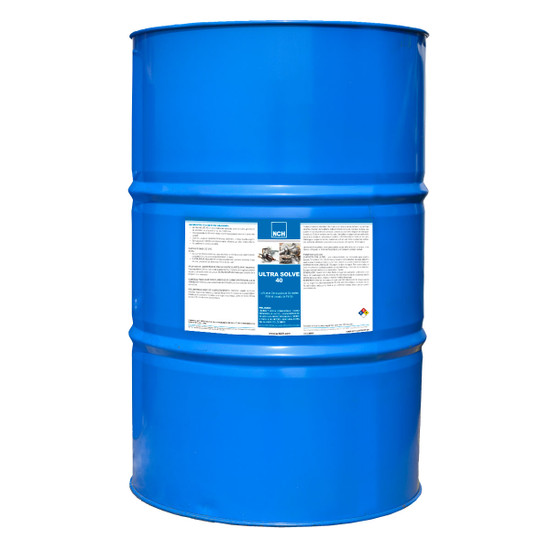
\includegraphics[scale=0.4]{images/Capitulo 4/s5/Contenedor/tambo_final.jpg}
            \caption{Contenedor de acero laminado propuesto}
            \label{fg:tambo}
        \end{figure}

Durante el funcionamiento del compostador el sistema se encontrará expuesto a las temperaturas del ambiente, puesto que ingresará aire del exterior por lo que en días fríos es probable que el contenedor experimente pérdidas de calor, esto se debe a que la temperatura del entorno es menor que la del sistema, cuando esto ocurre el calor tiende a fluir desde el sistema hacia el ambiente, con el fin de alcanzar un equilibrio térmico.
\newpage

Se parte de la ley de Fourier para la conducción de calor, la cual relaciona la cantidad de calor (Q) que atraviesa una pared de superficie (A), siendo K la constante de conductividad del material, y con una variación de temperatura ($\Delta$T) sobre un espesor ($\epsilon$).\cite{LeyFourier}

\begin{center}
    
    $Q = -AK\frac{\Delta T}{\Delta \varepsilon} $
\end{center}

Para las tapas del cilindro:

\[
Q = \frac{k2\pi r^2 (T_2 - T_1)}{\varepsilon}
\]

Por otro lado, la ley de Newton para la transferencia de calor establece que la tasa de transferencia de calor por convección entre un objeto sólido y un fluido es directamente proporcional a la superficie por la diferencia de temperaturas entre el fluido y el sólido.\cite{LeyNewtonCalor}

\[Q = h \cdot A \cdot \Delta T\]

Tomando en cuenta la expresión obtenida de la ley de Fourier y la ley de Newton para la transferencia de calor, se llega a la siguiente expresión:

\[T_f = \frac{\left(\frac{2\pi LKT_i}{\ln\left(\frac{r_0}{r_1}\right)} + hAT_{\text{aire}}\right)}{\left(hA+\frac{2\pi LK}{\ln\left(\frac{r_0}{r_1}\right)}\right)}\]

Se tomó el recopilado de las temperaturas registradas en el mes de enero (Figura \ref{fg:Tenero}), ya que es uno de los meses más fríos del año, presentando una temperatura mínima de tres grados Celsius.

\cite{TemperaturaEnero}
\begin{figure}[h!]
    \centering
        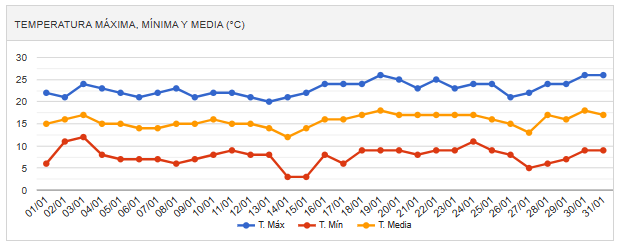
\includegraphics[scale=0.6]{images/Capitulo 4/s5/Contenedor/Temperaturas_Enero.png}
            \caption{Temperaturas registradas en enero del 2023 en la Ciudad de México}
                \label{fg:Tenero}
\end{figure}

Tomando en cuenta las expresiones previamente calculadas, y una temperatura de tres grados Celsius:
\[T_f = 322.97 \, \text{K}
\]
Se obtiene la potencia sustituyendo Tf en la ley de Fourier:


\[Q = 1.547 \, \text{kW}
\]


Se realizaron algunas simulaciones (estudios térmicos) en SolidWorks,  (Figura \ref{fg:Estermico}) para observar el comportamiento del contenedor bajo un escenario similar al que se propone teóricamente, en done se obtuvieron los siguientes resultados.
*****************************************************
\begin{table}
    \centering
    \resizebox{16cm}{!}{
    \begin{tabular}{|c|c|c|c|} 
    \hline
         Temperatura ambiental&  Temperatura interna contenedor&  Temperatura externa contenedor& Salida de potencia\\ \hline
         3° C&  50°C&  49.9°C& 1.54k W\\ \hline
         16°C&  50°C&  49.8°C& 1.12k W\\ \hline
         31.6°C&  50°C&  49.8°C& 604.81 W\\ \hline
    \end{tabular}
    }
    \caption{Caption}
    \label{tab:my_label}
\end{table}
En este primer estudio, es importante recalcar dos puntos, la temperatura externa del contenedor, es casi la misma que la temperatura interna del tambo, lo que en consecuencia podría representar un riesgo para quien manipule el dispositivo además de que esto generará grandes pérdidas de calor, como puede verse en la columna de "Salida de Potencia".
Tratando de contrarrestar este comportamiento que no es deseable para el funcionamiento del compostador se propone cubrir el contenedor un material aislante, en este caso se plantea utilizar fibra de vidrio, y se procedió a realizar  las simulaciones bajo los mismos parámetros, recubriendo las paredes externas con este nuevo material obteniendo los siguientes resultados:

***********************************************************************
\begin{table}
    \centering
    \resizebox{16cm}{!}{
    \begin{tabular}{|c|c|c|c|}
    \hline
         Temperatura ambiental&  Temperatura interna contenedor&  Temperatura externa contenedor& Salida de potencia\\ \hline
         3° C&  50°C&  6.2°C& 289.15 W\\ \hline
         16°C&  50°C&  18.2°C& 209.17 W\\ \hline
         31.6°C&  50°C&  32.8°C& 604.81 W\\ \hline
    \end{tabular}
    }
    \caption{Caption}
    \label{tab:my_label}
\end{table}

Como se puede observar, los resultados mejoraron considerablemente, puesto que las caras externas se encuentran cerca de 3 grados por encima de la temperatura ambiental propuesta, lo que permite mantener el calor al interior del contenedor, y en caso de que el usuario llegue a tocarlo, no se queme.
Añadiendo que, en los resultados obtenidos en la salida de  potencia  del modelo con fibra de vidrio, es cinco veces menor en comparación a la salida de potencia total del modelo sin aislante térmico, lo que permite observar una reducción significativa del calor transmitido.

